\section{Reference generation}
There are two ways for the user to interact with the \Multicopters: With a two joystick remote control (RC) or by sending various commands from the ground station PC.
The user inputs have to be transformed to yield corresponding reference values $(\rR, \RR, \vR, \wR, \vRd, \wRd)[k]$ for the \Multicopter controller.

The implemented procedure for doing so has two stages:
First the flatness of the \Multicopter models is exploited to reference values by a reference for the flat output with an intuitive interpretation.
If the RC is used, its joystick deflections have to be processed to yield the flat output components and their derivatives.
If the PC commands are used, they are processed to yield trajectories for the flat output.
%\ie $(y_\idxRef[k], \dot{y}_\idxRef[k], \ldots) \mapsto (\rR, \RR, \vR, \wR, \vRd, \wRd)[k]$.

\begin{itemize}
 \item Flatness
 \item Groundstation commands: Reference generation
 \item RC input: pilot supporting control
 \item Quadcopter integral action
\end{itemize}


\subsection{Flatness}\label{sec:RealizationRefGenFlatness}
For the discussion of flatness of the \Multicopter models we neglect the force and torque biases $\FB=0$ and $\tauB=0$.
Furthermore it is useful to express the models in terms of the translational velocity $\rd = \R \v$.

\paragraph{Tricopter.}
The \Tricopter model can be written as
\begin{subequations}\label{eq:RefGenTricopterModel}
\begin{align}
 \R^\top \R &= \idMat[3], \quad \det \R = +1,
\label{eq:RefGenTricopterGeoConstraint}
\\
 \Rd &= \R \wedOp(\w),
\\
 \J \dot{\w} + \wedOp(\w) \J \w &= \tau,
\\
 m(\rdd-\gravityAcc) + d \rd &= \R F.
\label{eq:RefGenTricopterTranslationalDyn}
\end{align}
\end{subequations}
Since the model is fully-actuated, any minimal parameterization of its configuration space is a flat output.
But since the configuration space is non-Euclidean, there is no global minimal parameterization.
In practice the \Tricopter cannot tilt too much anyway, so we will be content with a parameterization of the attitude $\R$ that is defined around the hover condition.

\paragraph{Quadcopter.}
For the \Quadcopter model we simply replace \eqref{eq:RefGenTricopterTranslationalDyn} by
\begin{align}
  m(\rdd-\gravityAcc) + d \rd = \R \ez \, \Fz.
\end{align}
The flatness of this model is extensively discussed in \cite{Konz:QuadrotorMovingFrame}.
From the number of inputs $\Fz \in \RealNum$ and $\tau \in \RealNum^3$ it is clear that a flat output has 4 components, i.e.\ $y \in \RealNum^4$.
We choose the position as the first 3 components $y_{1\ldots3} = r$ of the flat output.
From these we can already compute the total thrust $\Fz$ and the last column of the rotation matrix $\R$ as
\begin{align}\label{eq:RefGenQuadcopterConstraint}
 \Fz &= \pm \norm{m(\rdd-\gravityAcc) + d \rd},&
 \R \ez &= \sign(\Fz) \frac{m(\rdd-\gravityAcc) + d \rd}{\norm{m(\rdd-\gravityAcc) + d \rd}}.
\end{align}
Obviously this parameterization is singular for $\norm{m(\rdd-\gravityAcc) + d \rd} = 0$.
This singularity is intrinsic, i.e.\ it can not be avoided by a different parameterization.
A way to tackle this problem is discussed in \cite{Lenoir:2kPi}.

Here, due to practical limitations, we can only realize a strictly positive total thrust $0 < \FzMin \leq \Fz \leq \FzMax$ anyway.
So we don't need to worry about the singularity, if we ensure that the reference trajectory for the position obeys $\FzMin \leq \norm{m(\rdd-\gravityAcc) + d \rd} \leq \FzMax$.

The third column of the rotation matrix $\R$ is fixed by the first three components of the flat output $y_{1\ldots3} = r$ by \eqref{eq:RefGenQuadcopterConstraint}. 
So the remaining one degree of freedom of the rotation matrix has to be parameterized the remaining fourth component $y_4$ of the flat output.
This is a purely geometric problem:
Let $\Rx, \Ry, \Rz \in \RealNum^3$ be the columns of the rotation matrix, i.e.\ $\R = [\Rx,\Ry,\Rz]$.
The task is to find a continuous map $(y_4, \Rz) \mapsto (\Rx, \Ry)$ that obeys the geometric constraints \eqref{eq:RefGenTricopterGeoConstraint}.
Since the constraints imply $\Rz\times\Rx = \Ry$ we can eliminate $\Ry$ from the problem.
The reduced problem is to find a continuous map $(y_4, \Rz) \mapsto \Rx$ with the remaining constraints $\norm{\Rx} = 1$ and $\sProd{\Rz}{\Rx} = 0$.
Recall that $\Rz \in \RealNum^3$, $\norm{\Rz}=1$.
So geometrically the problem is finding a continuous unit vector field on the 2-sphere.
The \textit{hairy ball theorem} \cite{Brouwer:HairyBallTheorem} implies that any such vector field must have at least one singularity.
Even though unavoidable, this singularity is not intrinsic.
With a suitable parameterization of the rotation matrix $\R$ we can move it where it hurts least.

Any flat output $y_{1\ldots4}$ of the \Quadcopter supplemented with $y_5=\Fx$ and $y_6=\Fy$ is a flat output of the \Tricopter.

\paragraph{Rotation matrix decomposition.}
For $\varphi \in \RealNum$ and $\p = [\px,\py,\pz]^\top \in \Sphere^2 \backslash [0,0,-1]^\top$ we define the rotation matrices
\begin{align}
 \RotMatZ(\head) &=
 \begin{bmatrix}
  \cos\head & -\sin\head & 0 \\
  \sin\head & \cos\head & 0 \\
  0 & 0 & 1
 \end{bmatrix},&
 \RotMatPZ(\p) &=
 \begin{bmatrix}
  1 - \frac{(\px)^2}{1+\pz} & -\frac{\px \py}{1+\pz} & \px \\
  -\frac{\px \py}{1+\pz} & 1 - \frac{(\py)^2}{1+\pz} & \py \\
  -\px & -\py & \pz
 \end{bmatrix}.
\end{align}
The matrix $\RotMatZ$ is a rotation about the $\ez$ axis with angle $\head$ and $\RotMatPZ(\p)$ is a rotation about the axis $\ez \times p$ with the angle $\alpha = \cos^{-1} \pz$.
The matrix $\RotMatPZ$ can also be defined as the unique rotation matrix $\R$ that solves $\p = \R \ez$ and has the \textit{minimal angle} $\alpha = \cos^{-1} \tfrac{1}{2}(\tr \R - 1)$, see \cite{Konz:QuadrotorMovingFrame}.
In \autoref{fig:HairyBalls} the the three columns of $\RotMatPZ(\p)$ are illustrated as red, green and blue lines starting at the point $\p$ on the 2-sphere.
In particular it should illustrate the relation to the hairy ball theorem:
On the upper hemisphere the hair are combed quite well, whereas it gets more messy on the lower hemisphere with a cowlick at the southpole. 

% \begin{minipage}{\linewidth}
%  \centering
%  \input{graphics/IllustrateMinRotMat.pdf_tex}
%  \captionof{figure}{Illustration of $\RotMatZ(\head)$, left, and $\RotMatPZ(p)$, right}
%  \label{fig:IllustrateMinRotMat}
% \end{minipage}

%\begin{figure}[ht]
% 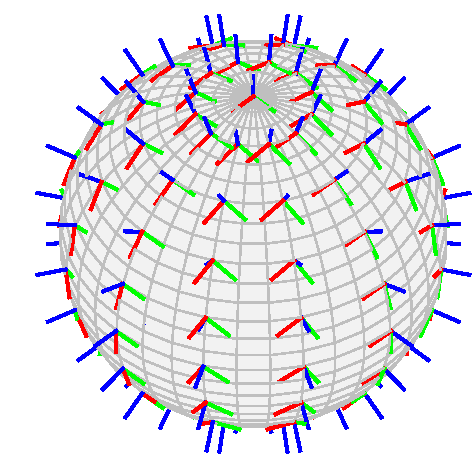
\includegraphics{HairyBall/HairyBallUpper.pdf}
% 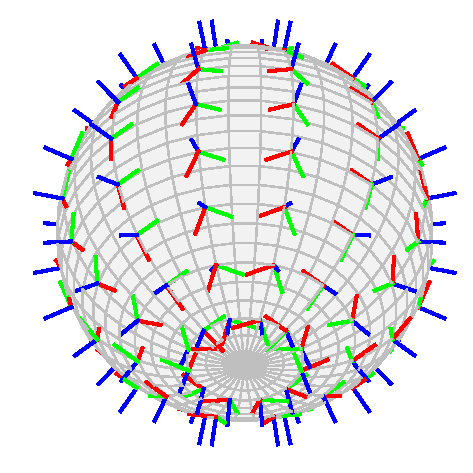
\includegraphics{HairyBall/HairyBallLower.pdf}
% \caption{Illustration of the rotation matrix $\RotMatPZ(\p)$}
% \label{fig:HairyBalls}
%\end{figure}

Combination of the matrices as $\R = \RotMatZ(\head) \RotMatPZ(\p)$ is a non-minimal parameterization of the rotation matrices $\SpecialOrthogonalGroup(3)$ except the ones for which $\R \ez = -\ez$.
This case would correspond to $\p = -\ez$ for which $\RotMatPZ$ is undefined.
The explicit relations for the entries of the rotation matrix $\R$ and the angular velocity $\w = \veeOp( (\RotMatZ(\head) \RotMatPZ(\p))^\top \tdiff{t} (\RotMatZ(\head) \RotMatPZ(\p)))$ are
\begin{subequations}
\begin{align}
 \begin{bmatrix} \Rxx & \Rxy & \Rxz \\ \Ryx & \Ryy & \Ryz \\ \Rzx & \Rzy & \Rzz \end{bmatrix}
 &=
 \begin{bmatrix}[1.2]
%   \cHeadR - \tfrac{\px (\cHeadR \px - \sHeadR \py)}{1+\pz} & -\sHeadR- \tfrac{\py (\cHeadR \px - \sHeadR \py)}{1+\pz} & \cHeadR \px - \sHeadR \py \\
%   \sHeadR - \tfrac{\px (\sHeadR \px + \cHeadR \py)}{1+\pz} &  \cHeadR- \tfrac{\py (\sHeadR \px + \cHeadR \py)}{1+\pz} & \sHeadR \px + \cHeadR \py \\
  \cHead - \tfrac{\px \px'}{1+\pz} & -\sHead - \tfrac{\py \px'}{1+\pz} & \px' \\
  \sHead - \tfrac{\px \py'}{1+\pz} &  \cHead - \tfrac{\py \py'}{1+\pz} & \py' \\
  -\px & -\py & \pz \\
 \end{bmatrix},
\qquad
 \left\{ \begin{array}{l} \px' = \cHead \px - \sHead \py \\ \py' = \sHead \px + \cHead \p \end{array} \right.
\\
 \begin{bmatrix} \wx \\ \wy \\ \wz \end{bmatrix}
 &=
 \begin{bmatrix}[1.2]
  0 & -1 & \tfrac{\py}{1+\pz} & -\px \\
  1 & 0 & -\tfrac{\px}{1+\pz} & -\py \\
  \tfrac{\py}{1+\pz} & -\tfrac{\px}{1+\pz} & 0 & \pz \\
 \end{bmatrix}
 \begin{bmatrix} \pxd \\ \pyd \\ \pzd \\ \headd \end{bmatrix}
% \\
%  \begin{bmatrix} \wxd \\ \wyd \\ \wzd \end{bmatrix}
%  &=
%  \begin{bmatrix}[1.2]
%   0 & -1 & \tfrac{\py}{1+\pz} & -\px \\
%   1 & 0 & -\tfrac{\px}{1+\pz} & -\py \\
%   \tfrac{\py}{1+\pz} & -\tfrac{\px}{1+\pz} & 0 & \pz \\
%  \end{bmatrix}
%  \begin{bmatrix} \pxdd \\ \pydd \\ \pzdd \\ \headdd \end{bmatrix}
%  +
%  \begin{bmatrix}
%   \frac{\pyd\pzd}{1+\pz} - \frac{\py\pzd^2}{(1+\pz)^2} - \pxd \headd \\
%   \frac{\px\pzd^2}{(1+\pz)^2} - \frac{\pxd\pzd}{1+\pz} - \pyd \headd \\
%   \frac{(\px\pyd - \py\pxd)\pzd}{(1+\pz)^2} + \pzd \headd \\
%  \end{bmatrix}
\end{align}
The inverse relations are
\begin{align}
 \varphi &= \atanTwo(\Ryx-\Rxy, \Rxx+\Ryy),
\quad 
 [\px, \py, \pz] = [-\Rzx, -\Rzy, \Rzz]
\\
 \begin{bmatrix} \pxd \\ \pyd \\ \pzd \\ \headd \end{bmatrix}
 &=
 \begin{bmatrix}
  0 & \Rzz & -\Rzy \\
  -\Rzz & 0 & \Rzx \\
  -\Rzy & \Rzx & 0 \\
  \tfrac{\Rxz}{1+\Rzz} & \tfrac{\Rzy}{1+\Rzz} & 1 \\
 \end{bmatrix}
 \begin{bmatrix} \wx \\ \wy \\ \wz \end{bmatrix}
\end{align}
\end{subequations}
It is also worth noting that the matrices $\RotMatZ(\head)$ and $\RotMatPZ(\p)$ obey the commutation law
\begin{align}\label{eq:CommutativityAttitudeDecompostion}
 \RotMatZ(\head) \RotMatPZ(\p) = \RotMatPZ(\RotMatZ(\head) \p) \RotMatZ(\head).
\end{align}


\subsection{Groundstation input}
In this mode the \Multicopter is in configuration control mode and receives commands from the groundstation.
Commands can be to start a precomputed trajectory or to compute 

We have 6 sufficiently smooth reference trajectories $t \mapsto y_{\idxRef i}, i=1,\ldots,6$.
The first 3 components are mapped to the position
\begin{align}
 \rRx = y_{\idxRef1}, \
 \rRy = y_{\idxRef2}, \
 \rRz = y_{\idxRef3}, 
\end{align}
For the attitude there are 3 different approaches implemented.

\paragraph{1.\ Tricopter mode.}
Let the reference attitude be decomposed as $\RR = \RotMatZ(\headR) \RotMatPZ(\pR)$ and the reference trajectories are mapped as
\begin{align}
 \headR = y_{\idxRef4},
 \pRx = y_{\idxRef5}, \
 \pRy = y_{\idxRef6}, \
\end{align}
The third component of $\pR$ is set to
\begin{align}
 \pRz = \sqrt{1 - (y_{\idxRef5})^2 - (y_{\idxRef6})^2}.
\end{align}
which restricts the reference attitude to $\pRz = \RRzz > 0$, but this is reasonable in practice:
Due to the limited propeller thrust on the \Tricopter, the reference tilts are limited to $|\pRx|, |\pRy| \leq 0.3$ anyway.

\paragraph{2.\ Quadcopter mode with heading angle.}
For the \Quadcopter we have 4 sufficiently smooth reference trajectories $t \mapsto y_{\idxRef i}, i=1,\ldots,4$.
We decompose the reference attitude by $\RR = \RotMatZ(\headR) \RotMatPZ(\pR)$ and set the inputs as
\begin{align}
 \headR = y_{\idxRef4}.
\end{align}
From \eqref{eq:RefGenQuadcopterConstraint} we get the tilt coefficients $\pR$ as
\begin{align}
 \pR = \RotMatZ^\top(\headR) \frac{m(\rRdd-\gravityAcc) + d\rRd}{\norm{m(\rRdd-\gravityAcc) + d\rRd}}
\end{align}

Note that swapping the order of heading and tilting rotations, i.e.\ parameterizing the attitude by $\RR' = \RotMatPZ(\pR') \RotMatZ(\headR)$, we get a different tilt vector
\begin{align}
 \pR' = \frac{m(\rRdd-\gravityAcc) + d\rRd}{\norm{m(\rRdd-\gravityAcc) + d\rRd}} = \RotMatZ(\headR) \pR.
\end{align}
But, due to the identity \eqref{eq:CommutativityAttitudeDecompostion}, the resulting attitude is the same $\RR' = \RR$.
This essentially means that we can interpret the reference heading angle $\headR$ in both ways, independent of how it actually defined.
%It should be stressed that this is a consequence of the particular definition of the tilt rotation $\RotMatPZ$.


\paragraph{Approach 3: Quadcopter mode with heading velocity.}
In some practical applications we just want to move the \Quadcopter around and do not really care about its heading.
Furthermore, as discussed in the previous subsection, any parameterization of the heading will result in a corresponding singularity.
Ultimately this limits the range of possible reference trajectories.
The previous approach for example, forbids reference trajectories in which the copter is upside down, $\RR \ez = -\ez$. 

A way to overcome this problem is to drop the parameterization of the heading.
Instead we parameterize the associated \textit{velocity} $\wRz$ and \textit{integrate} the remaining part $\RR \ex$ and $\RR \ey$ of the reference attitude.
Set the reference trajectories to
\begin{align}
 \rRx &= y_{\idxRef1},&
 \rRy &= y_{\idxRef2},&
 \rRz &= y_{\idxRef3},&
 \wRz &= y_{\idxRef4}.
\end{align}
Let $\RRx, \RRy, \RRz \in \RealNum^3$ be the columns of the reference rotation matrix, i.e.\ $\RR = [\RRx, \RRy, \RRz]$.
The reference attitude can be computed and integrated from
\begin{align}
 \RRz &= \frac{m(\rRdd-\gravityAcc) + d\rRd}{\norm{m(\rRdd-\gravityAcc) + d\rRd}},
\\
 \RRxd &= \wRz \RRy - \wRy \RRz,&
 \wRy &= \RRx^\top \RRzd
\\
 \RRyd &= \wRx \RRz - \wRz \RRx,&
 \wRx &= -\RRy^\top \RRzd.
\end{align}

%\paragraph{Example Trajectory.}
%\begin{figure}
% \centering
% 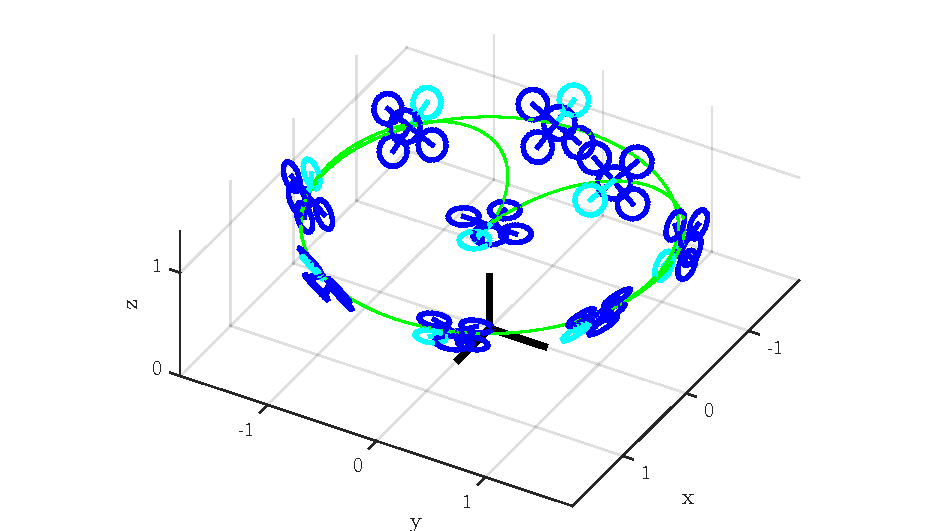
\includegraphics{QuadCircleTraj/QuadCircleTrajSnapshots}
%\\
% 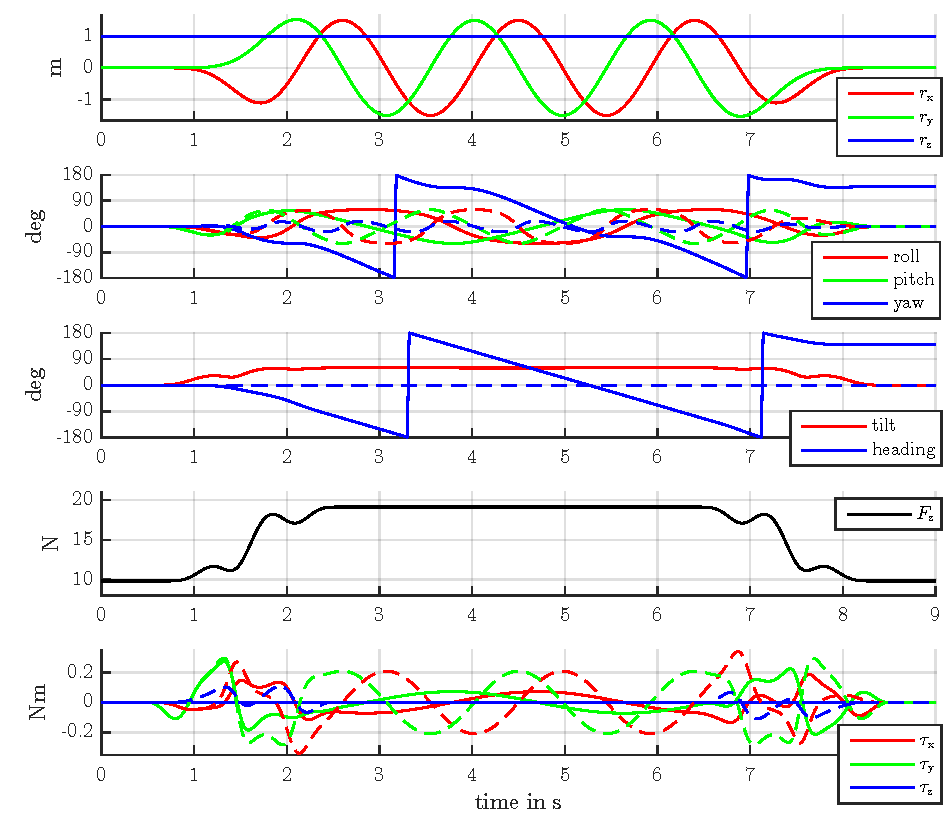
\includegraphics{QuadCircleTraj/QuadCircleTrajGraph}
% \caption{Example trajectory}
%\end{figure}



\subsection{Remote control input}
We use a standard remote control (FUTABA FX-35) with 8 analog channels and 6 switches, see \autoref{fig:RCchannels}.
On the multicopter side the receiver (FUTABA R6303SB) outputs the channels through the proprietary S.Bus which has been reverse engineered\footnote{\url{www.hackaday.com/2012/04/05/reverse-engineering-a-fubata-sbus-remote-control/}} to capture the channel values on the microcontroller.
The channels have a resolutions of $12\,\unit{Bit}$ and are sampled with $14\,\unit{ms}$.
The analog channels are scaled to the domain $-1 \leq \uRC[i] \leq 1, i=1\ldots,8$ and the switches to $\sRC[i] \in \{0,1,2\}, i=1,\ldots,6$.

%\begin{figure}[ht]
%\centering
% \input{graphics/RCchannels.pdf_tex}
% \caption{Remote control channels}
% \label{fig:RCchannels}
%\end{figure}

\paragraph{Derivative filtering.}
For the reference generation we need the derivatives of the analog RC inputs $\uRC$.
For this we implement the exact discretization (sampling time $\Ts=5\,\unit{ms}$) of a continuous filter of the from
\begin{align}
 \tdiff{t} \begin{bmatrix} \yRC[i] \\ \yRCd[i] \\ \yRCdd[i] \\ \yRCddd[i] \end{bmatrix}
 &= \begin{bmatrix} 0 & 1 & 0 & 0 \\ 0 & 0 & 1 & 0 \\ 0 & 0 & 0 & 1 \\ -a_0 & -a_1 & -a_2 & -a_3 \end{bmatrix}
 \begin{bmatrix} \yRC[i] \\ \yRCd[i] \\ \yRCdd[i] \\ \yRCddd[i] \end{bmatrix}
 + \begin{bmatrix} 0 \\ 0 \\ 0 \\ a_0 \end{bmatrix}
 \uRC[i],
\qquad 
 i = 1,\ldots,8.
\end{align}

The filter coefficients $a_i$ are chosen to resemble a (continuous) Bessel filter with cutoff frequency $7\,\unit{Hz}$, see e.g.\ \cite[sec.\,13.1.3]{TietzeSchenk:Halbleiter-Schaltungstechnik}.
A Bessel filter is characterized by having a maximally flat group delay, i.e.\ it preserves the (time-domain) shape of the signal in the passband (opposed to a Butterworth filter which preserves the amplitude in the frequency domain).
With rising order the (IIR) Bessel filter converges to a (FIR) Gaussian filter \cite[sec.\ 4.9.2]{Rabiner:DSP}.
\autoref{fig:RCFilter} shows the impulse response and application to a measured example RC-channel of the used Bessel filter and a corresponding Gaussian filter (windowlength 43).
Even though the difference is visible on the impulse response, the result of the implemented filter and the Gauss filter are indistinguishable in the application result.

%\begin{figure}[t]
% \centering
% 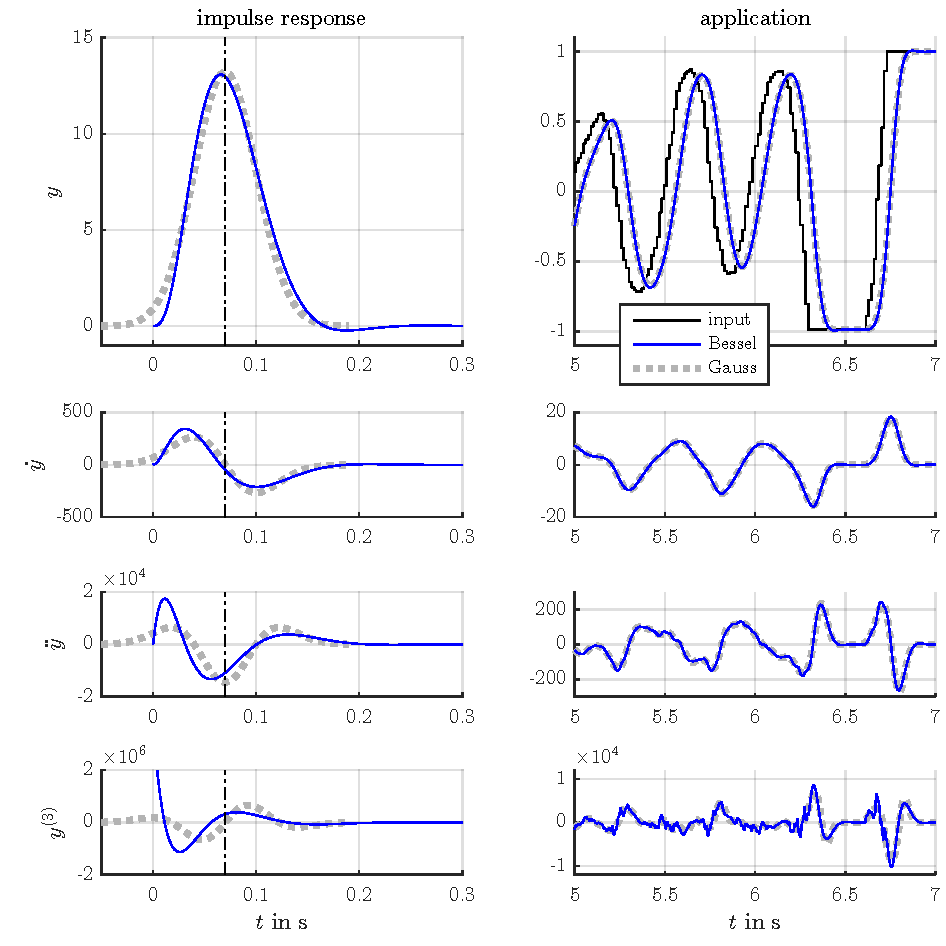
\includegraphics{RCFilter/RCFilter.pdf} 
% \caption{Application of the filter to the RC input}
% \label{fig:RCFilter}
%\end{figure}

The implemented filter is a trade-off between approximating the Gauss filter and being computationally cheap.

\subsection{Pilot mode}
In this mode the pilot commands the desired acceleration and attitude of the \Multicopter and 
\begin{align}
 \rRdd &= \RotMatZ(\headR) \accMax [\yRC[1], \yRC[2], \yRC[3]]^\top, 
\\
 \headRd &= \headRateMax \yRC[4],
\\
 \pRx &= \tiltMax \yRC[5], \ \pRy = \tiltMax \yRC[6],
\end{align}



\subsection{Trajectory generation modes}
\begin{itemize}
 \item Pilot mode without position control
 \begin{itemize}
  \item RC to acceleration in pilot frame
 \end{itemize}
 \item Pilot mode with position control
 \begin{itemize}
  \item RC to (integrated) position in pilot frame
 \end{itemize}
 \item Groundstation commands
 \begin{itemize}
  \item start polynomial transition to new position
  \item start precomputed trajectory
 \end{itemize}
\end{itemize}


%\begin{figure}[ht]
% \centering
% \input{graphics/IllustrateRCInputFrame.pdf_tex}
% \caption{Pilot reference frame}
% \label{fig:IllustrateRCInputFrame}
%\end{figure}


\paragraph{Transformation to reference signal.}
In pilot-mode only the remote control is used to interface with the multicopters.
One goal here is to establish an interface that works for the quadcopter \textit{and} the tricopter.

Firstly we only consider the outdoor operation where only the measurements from the IMU are available.
Here the body fixed force $F$ is computed from the RC inputs and the attitude $\R$ is actively controlled. 

To motivate the input scheme one has to put oneself into the pilots position:
The pilot knows the gravity $\vect{g}$ direction and sees the multicopter... \autoref{fig:IllustrateRCInputFrame}.
\begin{align}
 \rRdd = \RotMatZ(\headR) \pilotAccR
\qquad
 \RR = \RotMatZ(\headR)\, \RotMatPZ(\tiltCoeffR)
\end{align}
For the tricopter this yields the body fixed force
\begin{align}
 F_{\idxRef} = m \RRT (\rRdd - \gravityAcc) = m \RotMatPZ^\top(\tiltCoeffR) (\pilotAccR - \gravityAcc)
\end{align}



\begin{table}[ht]
\centering
\begin{tabular}{ccccc}
 \toprule
 quantity & scale & filter param & RC channel & comment\\
 \midrule
 $a_x$ & $\pm 3\,\sfrac{\unit{m}}{\unit{s}^2}$ & $70\,\unit{ms}$ & 1 \\
 $a_y$ & $\pm 3\,\sfrac{\unit{m}}{\unit{s}^2}$ & $70\,\unit{ms}$ & 0 \\
 $a_z$ & $\pm 3\,\sfrac{\unit{m}}{\unit{s}^2}$ & $70\,\unit{ms}$ & 2 \\
 $\dot{\varphi}$ & $\pm 60\,\sfrac{\unit{DEG}}{\unit{s}}$ & $150\,\unit{ms}$ & 3 \\
 $p_x$ & $\pm \sfrac{1}{3}$ & $150\,\unit{ms}$ & 10 & only tricopter \\
 $p_y$ & $\pm \sfrac{1}{3}$ & $150\,\unit{ms}$ & 11 & only tricopter \\
 \bottomrule
\end{tabular}
\caption{Pilot interface}
\label{tab:PilotInterface}
\end{table}


\subsection{Integral action for Quadcopter}
So far we have neglected the bias forces and torques $\FB$ and $\tauB$ for reference generation.
For the \Tricopter this is fine since they do not affect possible reference trajectories $t \mapsto (\rR, \RR)(t)$.
For any bias force and torque there is a control force that can counteract to it.

For the \Quadcopter the situation is different:
There are no control forces that directly counteract to $\FBx$ and $\FBy$.
Practically one can easily imagine that if the \Quadcopter should hover, $\rR=\const$, in the presence of a side wind it has to tilt to compensate it.
Mathematically this means that \eqref{eq:RefGenQuadcopterConstraint} is not valid for $\FBx, \FBy \neq 0$.

Introduce $\RR'$ and $\FRz'$ as the corrected reference that fulfill the translational dynamics in the presence of bias force
\begin{align}
 m(\rRdd-\gravityAcc) + d \rRd = \RR' (\FRz' \ez + \FB).
\end{align}
Set $\RR' = \RR P$, where $P\in \SpecialOrthogonalGroup(3)$ is the correction.
Using the properties of the nominal reference from \eqref{eq:RefGenQuadcopterConstraint} we can write
\begin{align}
 \underbrace{\RRT \big( m(\rRdd-\gravityAcc) + d \rRd \big)}_{\FRz \ez} = P (\FRz' \ez + \FB).
\end{align}
Decomposing this into magnitude and direction we have
\begin{align}\label{eq:RefGenQuadIntegralP}
 \FRz' = \sqrt{\FRz^2 - \FBx^2 - \FBy^2} - \FBz,
\qquad
 P^\top \ez = \tfrac{\FRz' \ez + \FB}{\FRz}.
\end{align}
This is a similar situation as discussed above for \eqref{eq:RefGenQuadcopterConstraint}: The relation \eqref{eq:RefGenQuadIntegralP} only fixes two of the three degrees of freedom of $P\in\SpecialOrthogonalGroup(3)$.
So we chose a similar solution
\begin{align}
 P^\top = \RotMatPZ\big( \tfrac{\FRz' \ez + \FB}{\FRz} \big).
\end{align}
This essentially is the solution of \eqref{eq:RefGenQuadIntegralP} for which the angle $\measuredangle P = \cos^{-1} \tfrac{1}{2}(\tr P - 1)$ is minimal.

By differentiation we get the corrected angular velocity $\wR' = \veeOp\big( (\RR P)^\top \tdiff{t}(\RR P)\big)$ and its derivative $\wRd'$.
This requires the assumption that the bias force is constant, $\FBd = 0$.

% For small bias force $\norm{\FB} \ll |\FRz|$ the corrections can be approximated as
% \begin{align}
%  \FRz' &= \FRz - \FBz + \mathcal{O}(\norm{\FB}^2),&
%  P &= \begin{bmatrix} 1 & 0 & -\tfrac{\FBx}{\FRz} \\ 0 & 1 & -\tfrac{\FBy}{\FRz} \\ \tfrac{\FBx}{\FRz} & \tfrac{\FBy}{\FRz} & 1 \end{bmatrix} + \mathcal{O}(\norm{\FB}^2).
% \end{align}
